\chapter{Johnson-Rauschen}
In diesem Teil des Experiments wird das Johnson- oder thermische Rauschen untersucht. Dieses Rauschen entsteht durch die thermisch bedingte Bewegung freier Elektronen in ohmschen Widerständen. 
Die Bewegung von Elektronen ist aufgrund zufälliger thermischer Energie ungeordnet und wird daher durch die statistische Physik beschrieben. In einem unbelasteten Stromkreis bewegen sich freie Elektronen ohne äußere Einflüsse zufällig, was zu Impulsübertragung und unabhängigen Spannungs- und Stromschwankungen führt. Diese überlagern sich und bilden das sogenannte weiße Rauschen.

Weißes Rauschen zeichnet sich durch eine gleichmäßige Leistungsverteilung über alle Frequenzen aus.
Das Johnson-Rauschen ist ein Sonderfall dieses Phänomens und lässt sich durch die thermische Bewegung von Elektronen in einem Leiter erklären. Die effektive Spannung $\langle V^2 \rangle$, die sich bei einer Temperatur T an einem Widerstand R einstellt, wird durch die Nyquist-Relation \cite{Nyquist} beschrieben:
\begin{equation}
\langle V^2 \rangle = 4 k_B T R \Delta f,
\end{equation}
wobei $k_B$ die Boltzmann-Konstante und $\Delta f$ die betrachtete Frequenzbandbreite darstellt.
%=======================================================================================================
\section{Aufbau}
\FloatBarrier
\begin{figure}[htbp]
    \centering
    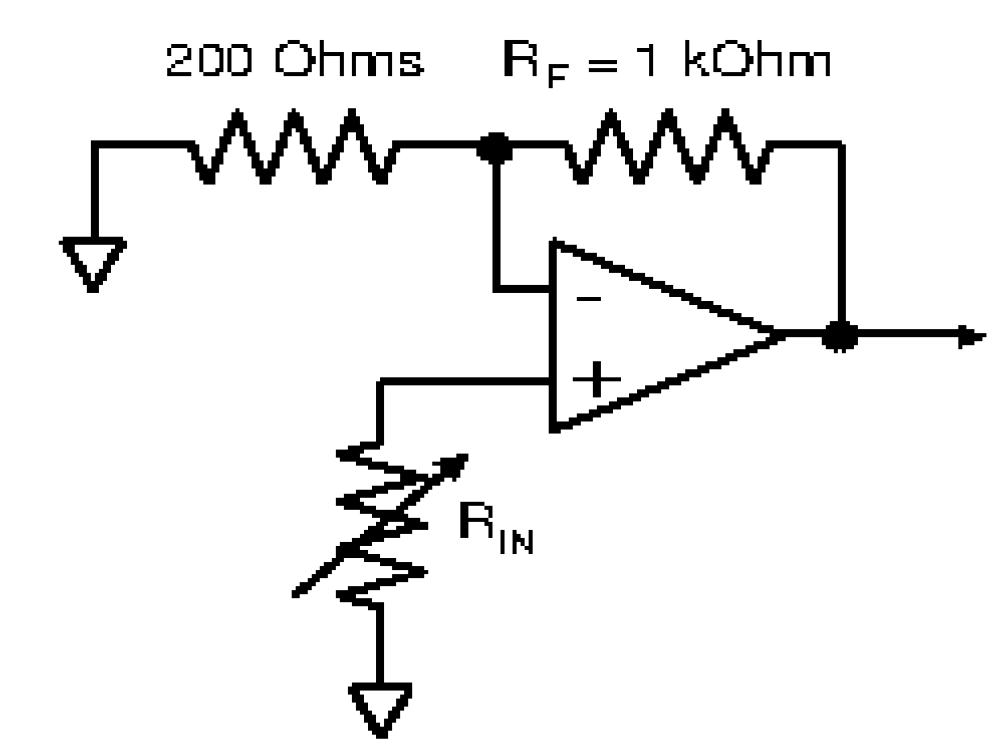
\includegraphics[width=0.5\textwidth]{figs/schalt amplifier.png}
    \caption{Schaltplan des Vorverstärkers der LLE-Box zur Messung des JohnsonRauschens \cite{praktikum}}
    \label{fig:schaltamplifier}
\end{figure}
\FloatBarrier
Da Johnson-Rauschen eine sehr geringe Signalstärke aufweist, ist eine spezielle Verstärkerschaltung erforderlich, um es sichtbar zu machen. Diese ist in Abbildung \ref{fig:schaltamplifier} dargestellt. Es handelt sich um einen nichtinvertierenden Verstärker, integriert in einer sogenannten LLE-Box (Low Level Electronics). Der vollständige Schaltplan ist in Abbildung \ref{fig:johnson lle} dargestellt.
\FloatBarrier
\begin{figure}[htbp]
    \centering
    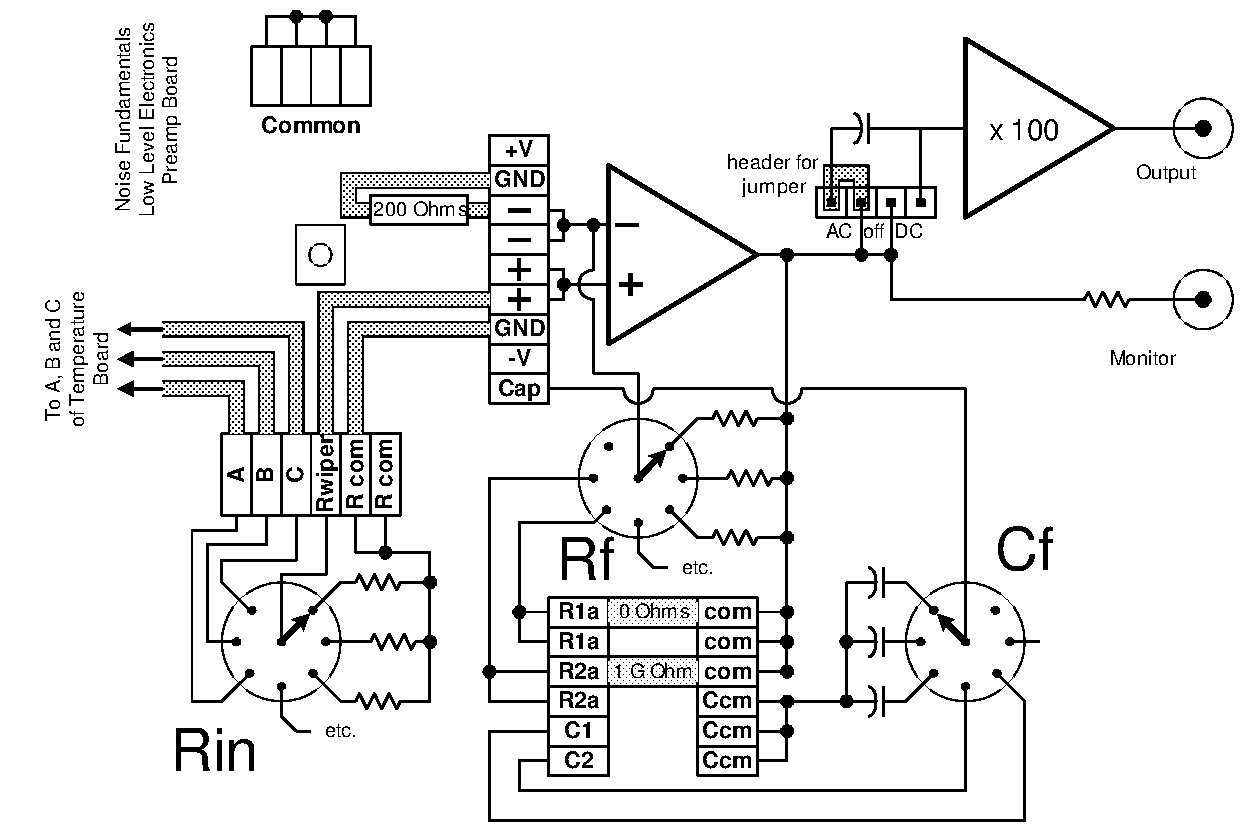
\includegraphics[width=0.75\textwidth]{figs/johnson lle.png}
    \caption{Interner Schaltplan der LLE-Box zur Messung des Johnson-Rauschens \cite{praktikum}}
    \label{fig:johnson lle}
\end{figure}
\FloatBarrier
Nach der Vorverstärkung gelangt das Signal in die HLE-Box (High-Level Electronics, Abbildung \ref{fig:johnson hle}), wo ein Bandpassfilter die relevanten Frequenzbereiche gezielt herausfiltert. Der Ausgang des Vorverstärkers wird dazu über ein BNC-Kabel mit dem Filtereingang der HLE-Box verbunden. Ein zweiter Filter in der HLE-Box ermöglicht die Implementierung eines zusätzlichen Bandpassfilters.
\FloatBarrier
\begin{figure}[htbp]
    \centering
    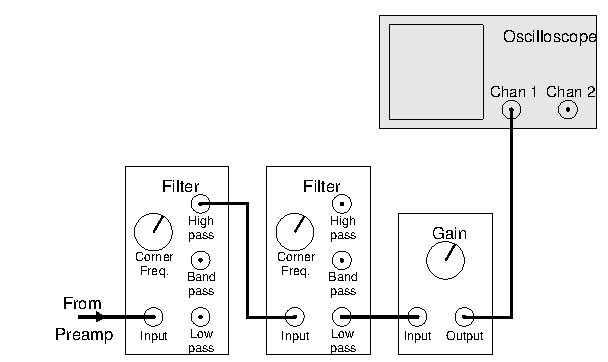
\includegraphics[width=0.5\textwidth]{figs/johnson hle.png}
    \caption{Schaltung der HLE-Box zum Visualisieren des Johnson-Rauschens \cite{praktikum}}
    \label{fig:johnson hle}
\end{figure}
\FloatBarrier
%========================================================================================================
\section{Durchführung und Auswertung}
%---------------------------------------------------------------------------------------------------
\subsection{Beobachten des Johnson-Rauschens}
Die Widerstände der LLE-Box sind auf $R_{in} = 100 k\Omega$  und $R_f = 1 k\Omega$ eingestellt, und die Verstärkung des Signals beträgt G = 600. Das Rauschen wird über einen Oszilloskop-Ausgang mit den Einstellungen $2\,\text{mV/div} \,, \quad 10\,\mu\text{s/div} \,, \quad \text{Triggerlevel} \approx 0$ und einer Eingangsimpedanz von $1\,\text{M}\Omega$ beobachtet. Die Grenzfrequenz des Hochpasses wird auf $f_{gr} = 0,1 kHz$, die Grenzfrequenz des Tiefpasses auf $f_{gr} = 100 kHz$, und der Gain wird auf $G_2 = 300$ eingestellt, um das Johnson-Rauschen zu isolieren. Die Messung erfolgt bei Raumtemperatur, um die thermischen Effekte zu berücksichtigen. Das Rauschen wird in Form eines zeitlichen Verlaufs auf dem Oszilloskop dargestellt, wobei die Amplitude des Rauschens in Millivolt und die Zeit in Mikrosekunden angegeben sind.
 beobachtet. 
 \FloatBarrier
\begin{figure}[htbp]
    \centering
    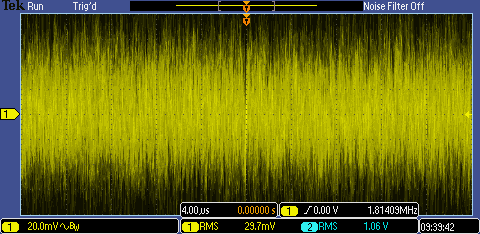
\includegraphics[width=0.5\textwidth]{figs/johnson_noise_without_filter.png}
    \caption{}
    \label{fig:johnson noise}
\end{figure}
\FloatBarrier

\begin{figure}[htbp]
    \centering
    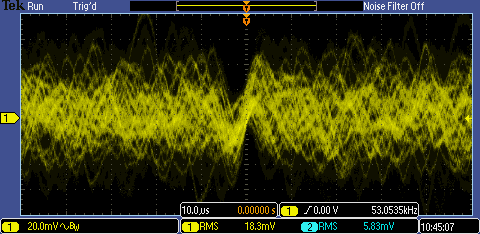
\includegraphics[width=0.5\textwidth]{figs/johnson noise with bandfilter.PNG}
    \caption{}
    \label{fig:bandfilter}
\end{figure}
\FloatBarrier
%---------------------------------------------------------------------------------------------------
\subsection{Messung des Johnson-Rauschens}
Zur Messung des Johnson-Rauschens wird ein Widerstand mit einem Wert von 1 k$\Omega$ verwendet. Dieser Widerstand wird in die Schaltung integriert, wie in Abbildung \ref{fig:johnson messung} gezeigt. Der Widerstand ist mit der HLE-Box verbunden, und das Rauschen wird über einen Oszilloskop-Ausgang beobachtet. Die Verstärkung des Signals beträgt G = 600, und die Bandbreite des Filters ist auf 10 kHz eingestellt.
\FloatBarrier
\begin{figure}[htbp]
    \centering
    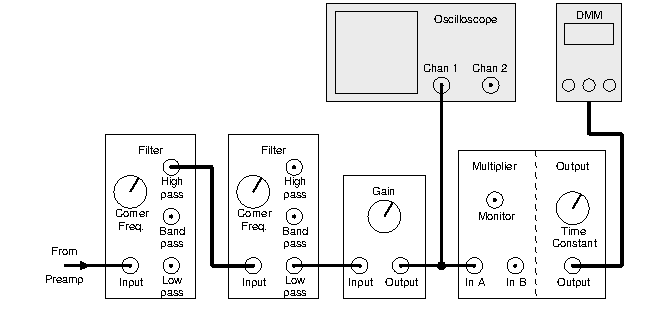
\includegraphics[width=0.5\textwidth]{figs/johnson hle and dmm.png}
    \caption{Verkabelung zur Messung des Johnson-Rauschens \cite{praktikum}}
    \label{fig:johnson messung}
\end{figure}
\FloatBarrier

\begin{figure}[htbp]
    \centering
    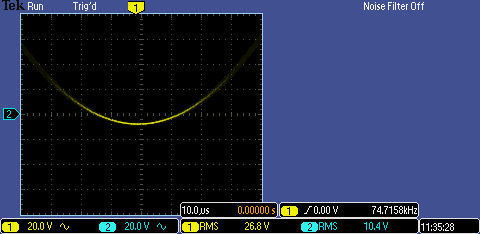
\includegraphics[width=0.5\textwidth]{figs/johnson parabel.png}
    \caption{}
    \label{fig:parabel}
\end{figure}
\FloatBarrier
%---------------------------------------------------------------------------------------------------
\subsection{Abhängigkeit des Johnson-Rauschens vom Widerstand}
%---------------------------------------------------------------------------------------------------
\subsection{Abhängigkeit des Johnson-Rauschens von der Bandbreite}
%---------------------------------------------------------------------------------------------------
\subsection{Bestimmung der Bolzmann-Konstante}